\documentclass{aip-cp}

\usepackage[numbers]{natbib}
\usepackage{rotating}
\usepackage{graphicx}

\usepackage{bm}

%\makeatletter
%\def\@fnsymbol#1{\ensuremath{\ifcase#1\or *\or \dagger\or **\or
%   \ddagger\or \mathsection\or \mathparagraph\or \|\or \dagger\dagger
%   \or \ddagger\ddagger \or\mathsection\mathsection
%   \or \mathparagraph\mathparagraph \or *{*}*\or
%   \dagger{\dagger}\dagger \or\ddagger{\ddagger}\ddagger\or
%   \mathsection{\mathsection}\mathsection
%   \or \mathparagraph{\mathparagraph}\mathparagraph \else\@ctrerr\fi}}
%\makeatother

% Document starts
\begin{document}

% Title portion
\title{Algorithm of Time Step Evaluation for Numerical Solution of Boundary Value Problem for Parabolic  Equations}

%\author[aff1]{Author's Name\corref{cor1}\noteref{note1,note2}}
%\eaddress[url]{http://www.aip.org}
%\author[aff2,aff3]{Author's Name\noteref{note2}}
%\eaddress{anotherauthor@thisaddress.yyy}

\author[aff1,aff2]{Petr Vabishchevich}
\author[aff1,aff2]{Aleksandr Vasilev\corref{cor1}}

\affil[aff1]{Nuclear Safety Institute of RAS, Moscow, Russia}
\affil[aff2]{North-Eastern Federal University, Yakutsk, Russia}
\corresp[cor1]{Corresponding author: haska87@gmail.com}

\maketitle


\begin{abstract}
In this work the algorithm of automatic time step evaluation for solving
the boundary value problem for parabolic equations is proposed.
The solution is obtained using evaluation approach and fully implicit schemes.
The time step evaluation formulas are derived on the basis of the approximation error estimation at next time step.
Reliability of the proposed algorithm is demonstrated using the model problem calculations.
\end{abstract}

% Head 1
\section{INTRODUCTION}
For the second order parabolic equations unconditionally stable schemes are constructed on the basis of implicit approximations \cite{SamarskiiMatusVabischevich2002}.
In computational practice two-layer schemes are mostly used; three-layer and multilayer schemes are not so often used.
The problem of the time step control is relatively well developed for the Cauchy problem for differential equations systems \cite{Gear1971,ascher1998computer,HairerNorsettWanner1987}. 
The basic approach is based on using additional calculations at a new time step to estimate the approximate solution.
The time step is estimated using the theoretical asymptotic dependences of the accuracy on time step \cite{vabishchevich2015priori}.

Additional calculations for estimating the error of the approximate solution can be carried out in different ways. The best-known strategy is connected the calculation at separate time interval using the given time step (the first solution) and the half step (the second solution). The noted ways to evaluate the time step are related to methods of a posteriori accuracy estimation.
The decision to change or not the time step is accepted only after the calculation is completed.

In this paper, we consider a priori evaluation of the time step to obtain approximate solution of boundary value problems for parabolic equations. The calculation results for the model problem for parabolic equations demonstrate the reliability of the proposed time stepping algorithm.

\section{PROBLEM DESCRIPTION}
Consider the second-order parabolic equation
\begin{equation}\label{1}
   \frac{\partial u}{\partial t} 
   - \sum_{\alpha =1}^{m}
   \frac{\partial }{\partial x_\alpha} 
   \left ( k({\bm x},t)  \frac{\partial u}{\partial x_\alpha} \right ) + s({\bm x},t) u = f({\bm x},t),
   \quad {\bm x}\in \Omega,
   \quad 0 < t \leq  T,
\end{equation}
where
$\underline{k} \leq k({\bm x}) \leq  \overline{k}, \ {\bm x} \in \Omega, \ \underline{k} > 0$.
The equation (\ref{1}) is supplemented by boundary  condition
\[
   u({\bm x},t) = g({\bm x},t),
   \quad {\bm x}\in \partial \Omega,
   \quad 0 < t \leq  T,
\]
and initial condition
\[
   u({\bm x},0) = u^0({\bm x}),
   \quad {\bm x}\in \Omega.
\]
After spatial discretization (by the method of finite differences or finite elements) we consider the Cauchy problem
\begin{equation}\label{2}
\frac{du}{dt} + A(t)u =f(t), \quad 0 < t \leq T,
\end{equation}
with initial condition $u(0) = u^0$. 
The problem is considered in a finite-dimensional Hilbert space.
We assume that $A(t) \geq 0$.
Let's use an irregular time grid
\[
t^0 = 0, \quad t^{n+1} = t^n + \tau^{n+1}, \quad 
n = 0, 1, ... , N-1, \quad t^N = T.
\]
For the approximate solution the implicit scheme 
\begin{equation}\label{3}
  \frac{y^{n+1} - y^{n}}{\tau^{n+1}} + A^{n+1} y^{n+1} = f^{n+1},
  \quad n = 0,1, ..., N-1
\end{equation}
is used and initial condition 
$
y^0 = u^0 .
$
For the approximate solution we can use the following estimate
\[
 \|y^{n+1}\| \leq \|y^{n}\| + \tau^{n+1} \|f^{n+1}\| .
\]
Then we can obtain a difference analogue of the estimate for problem (\ref{3})
\begin{equation}\label{4}
 \|y^{n+1}\| \leq \|u^{0}\| + \sum_{k=0}^{n} \tau^{k+1} \|f^{k+1}\|.
\end{equation}
For the error of the approximate solution $z^n = y^n - u^n$ we have
\[
  \frac{z^{n+1} - z^{n}}{\tau^{n+1}} + A^{n+1} z^{n+1} = \psi^{n+1},
  \quad n = 0,1, ..., N-1,  \quad
 z^0 = 0.
\]
The approximation error $\psi^{n+1}$ is defined as
\begin{equation}\label{5}
 \psi^{n+1} = f^{n+1} -
 \frac{u^{n+1} - u^{n}}{\tau^{n+1}} - A^{n+1} u^{n+1} . 
\end{equation}
Similarly (\ref{4}), we obtain the estimate for the error
\begin{equation}\label{6}
  \|z^{n+1}\| \leq \sum_{k=0}^{n} \tau^{k+1} \|\psi^{k+1}\| .
\end{equation} 

Checking the error we can focus on the total error $\delta\tau^{n+1}$ in interval $t^n < t < t^{n+1}$. Then from (\ref{6}) we obtain
$\|z^{n+1}\| \leq \delta t^{n+1}.$
The error is accumulated and increases linearly.
The solution is obtained using the unconditionally stable implicit scheme.
The major part of computational capability are related with this scheme.
The step control is performed using the solution produced by explicit scheme.
The algorithm stability is not violated and determined by the implicit scheme properties.
The error accumulation from the time layer $t^n$ to the new layer $t^{n+1}$  is defined as
\begin{equation}\label{7}
\|z^{n+1}\| \leq \|z^{n}\| + \tau^{n+1} \|\psi^{n+1}\| .
\end{equation}
Therefore, we must control the local error $\psi^{n+1}$. Comparing $\psi^{n+1}$ with a given level of error $\delta$ we can control the evaluation of the time step. If $\psi^{n+1}$ is significantly larger (or smaller) then the $\delta$ -- it means that the time step is too large (or small). Thereby
\begin{equation}\label{8}
  \tau^{n+1}: \ \|\psi^{n+1}\| \approx \delta .
\end{equation} 

Consider the basic algorithm of time step evaluation. We select the time step based on the analysis of the solution at the previous step. The predicted time step is determined as following
\begin{equation}\label{9}
 \widetilde{\tau}^{n+1} = \gamma \tau^n , 
\end{equation}
where $\gamma$ is a numerical parameter. The default value of $\gamma$ is 1.25 or 1.5. Using the explicit scheme we can obtain a solution $\widetilde{y}^{n+1}$ at time $\widetilde{t}^{n+1} = t^n + \widetilde{\tau}^{n+1}$. The calculation is performed only at single time step. Therefore, the possible computational instability doesn't appear.
We estimate the approximation error using the calculated $\widetilde{y}^{n+1}$ by the implicit scheme. The $\tau^{n+1}$ is estimated by the proximity of the error norm to $\delta$. The solution at a new time step $t^{n+1}$ is calculated with a $\tau^{n+1}$  by the implicit scheme.

% Head 2
\section{CALCULATION FORMULAS}
We present the calculated formulas for the time step control. 
The predictive solution $\widetilde{y}^{n+1} $  is defined from
\[
  \frac{\widetilde{y}^{n+1} - y^{n}}{\widetilde{\tau}^{n+1}} + A^{n} y^{n} 
  = f^{n} .
\]
In accordance with (\ref{5}), the approximation error is calculated from the exact solution for two time moments: for $t^n$ and $\widetilde{t}^{n+1}$.
To estimate the error we take $u(t^n)$ instead of $y^n$. An exact solution at a new time step $u(\widetilde{t}^{n+1})$, is matched by an approximate solution $u(\widetilde{t}^{n+1})$, which is obtained by the explicit scheme. By virtue of this, we have
\begin{equation}\label{10}
 \widetilde{\psi}^{n+1}  = \widetilde{f}^{n+1} -
 \frac{\widetilde{y}^{n+1} - y^{n}}{\widetilde{\tau}^{n+1}} -
 \widetilde{A}^{n+1} \widetilde{y}^{n+1} . 
\end{equation} 
We match the approximation error $\widetilde{\psi}^{n+1}$ at the time step $\widetilde{\tau}^{n+1}$ and $\psi^{n+1}$ at the time step $\tau^{n+1}$.
Taking into account (\ref{8}), we obtain
\begin{equation}\label{11}
  \bar{\tau}^{n+1} = \gamma_{n+1} \tau^n,
  \quad \gamma_{n+1} = \frac{\delta}{\| \widetilde{\psi}^{n+1}\|}  \gamma.
\end{equation} 
Time step can not exceed the predicted time step, therefore
\[
\tau^{n+1} \leq \bar{\tau}_{n+1}, \quad \tau^{n+1} \leq \widetilde{\tau}_{n+1}.
\] 
We limit the allowable time step by the minimum step $\tau^0$
\begin{equation}\label{12}
 \tau^{n+1} = \max \big \{\tau^0, \min \{\gamma_{n+1}, \gamma \} \tau^n \big \}. 
\end{equation}
The calculation formulas for the step evaluation algorithm in accordance with (\ref{10})-(\ref{12}) defined as
\[
 \widetilde{\psi}^{n+1} = \widetilde{\tau}^{n+1} \left( \frac{\widetilde{f}^{n+1} - f^n}{\widetilde{\tau}^{n+1}}  - \frac{\widetilde{A}^{n+1} - A^n}{\widetilde{\tau}^{n+1}}  y^n - \widetilde{A}^{n+1} \frac{\widetilde{y}^{n+1} - y^n}{\widetilde{\tau}^{n+1}}  \right ) .
\] 
Thus the approximation error has the first order for
time variable
$
 \widetilde{\psi}^{n+1} = \mathcal{O} (\widetilde{\tau}^{n+1}) .
$ 
By virtue of this, we have 
\begin{equation}\label{13}
 \|\widetilde{\psi}^{n+1} \| \leq \|\widetilde{f}^{n+1} - f^n  -
 (\widetilde{A}^{n+1} - A^n) y^n -
 \widetilde{A}^{n+1} (\widetilde{y}^{n+1} - y^n) \| .
\end{equation} 
Taking into account (\ref{13}) and (\ref{11}) we obtain the calculated formula for time step (\ref{12}) in which
\begin{equation}\label{14}
  \gamma_{n+1} = \frac{\delta}{ \|\widetilde{f}^{n+1} - f^n  -
  (\widetilde{A}^{n+1} - A^n) y^n  -
  \widetilde{A}^{n+1} (\widetilde{y}^{n+1} - y^n) \| } \gamma .
\end{equation} 
This formula (the denominator of the expression) clearly shows the corrective actions which are associated with the change of the right-hand side (the first part) and the problem operator (the second part) and with the dynamics of the solution (the third part).

Similar formalas for the time step evaluation were obtained earlier in the papers \cite{vabishchevich2015priori, vabishchevich2015time} on the basis of an estimate of the change in the approximate solution. This method uses  two auxiliary steps with a predictable time step.
The first step is performed according to the explicit scheme, the second one -- according to the explicit scheme backwards.
Here we rely on a simpler and more general procedure for estimating the approximation error at the predicted time step according to the approximate by explicit scheme.

\section{TEST PROBLEM}
In this section, we present a numerical test to illustrate the efficiency of the algorithm. We solve the boundary-value problem for a one-dimensional parabolic equation
\begin{equation}\label{15}
  \frac{\partial u}{\partial t} - \frac{\partial^2 u}{\partial x^2} + p(t) u = f(t),
  \quad 0 < x < 1,
  \quad 0 < t \leq  T ,  
\end{equation}
with boundary and initial conditions
\begin{equation}\label{16}
  u(0, t) = 0,
  \quad u(1,t) = 0,
  \quad 0 < t \leq  T , 
\end{equation}
\begin{equation}\label{17}
  u(x,0) = u^0(x),
  \quad  \quad 0 <  x <  1 .
\end{equation}
For an approximate solution of the problem (\ref{15})-(\ref{17}) we use the finite-difference approximation with respect to space. 
Define the uniform grid with step $h$ as following
\[
  \bar{\omega} = \{ x \ | \ x = ih, \quad i = 0, 1, ..., M, \quad Mh = 1 \},  
\] 
where $\omega$ -- set of internal nodes, $\partial\omega$ -- set of boundary nodes ($\bar{\omega } = \omega \cup \partial \omega$).
On the set of grid functions $u(x) = 0, \ x \notin \omega$  we define a Hilbert space $H$, where the scalar product and norm is defined as
\[
 (u,v) = \sum_{x \in \omega} u(x) v(x) dx,
 \quad \|u\| = (u,u)^{1/2} . 
\]
The grid operator $ A (t) $ is defined as
\[
 A u = - \frac{1}{h^2} (u(x+h) - 2 u(x) + u(x-h)) + p(t) u(x),
 \quad x \in \omega . 
\]
The operator $A(t)$ is self-adjoint and for $p(t)\geq 0$ it is positive defined in $H$.
Thus, after spatial discretization from (\ref{15})-(\ref{17}) we obtain the problem (\ref{1}).
The problem (\ref{15})-(\ref{17}) is considered for $T = 0.1$ with the discontinuous coefficient $p(t)$ and the discontinuous right-hand side $f(t)$:
\[
  p(t) = \{\lambda  t: \ 0 < t \leq 0.075;\quad 0: \ 0.075 < t \leq 0.1  
  \}, 
\]
\[
  f(t) = \{0: \ 0 < t \leq 0.05; \quad \chi  e^{-10 (t-0.05)}: \ 0.05 < t \leq 0.1 \} .
\]
First, we consider the case when the initial condition (\ref{17}) is defined as
\[
  u^0(x) = \sin^\sigma (\pi x),
  \quad  \quad 0 <  x <  1 .
\]
For the basic variant set
\[
 \lambda = 100,
 \quad \chi = 10, 
 \quad \sigma = 0.5 . 
\]
The problem is solved on the grid $M = 100$ and the calculations are carried out with a small initial time step: $\tau^1 = \tau^0 = 1 \cdot 10^{-6}$. 

\begin{figure}[h]
    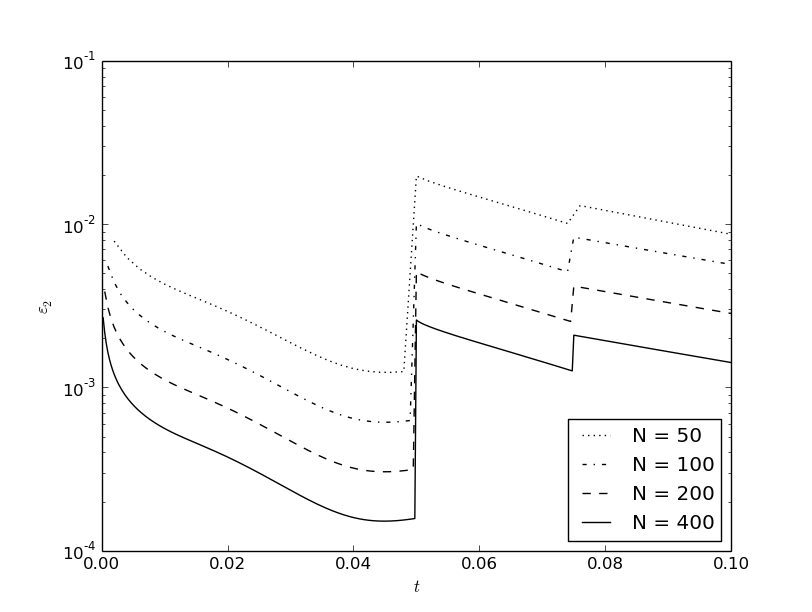
\includegraphics[width=0.5\linewidth] {art/1-1.png}
    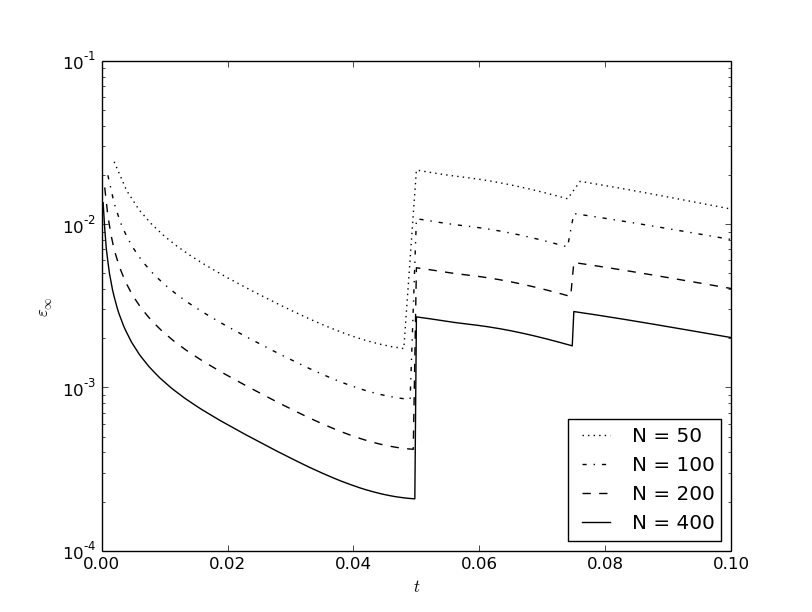
\includegraphics[width=0.5\linewidth] {art/1-2.png}
	\caption{The error in $L_2(\omega)$ and $L_\infty(\omega)$ on a uniform grid}
	\label{fig:1}
\end{figure} 

In this paper, we consider the problems of time discretization and therefore the spatial grid does not change. 
The accuracy of the approximate solution was estimated from the reference solution that we use as a numerical solution on a sufficiently detailed time grid ($\tau = 1 \cdot 10^{-7}$). 
The error is estimated in the norm of $L_2(\omega)$ ($\varepsilon_2 = \| \cdot \|$) or $L_\infty(\omega)$ ($\varepsilon_\infty = \| \cdot \|_\infty$), and
\[
 \| u \|_\infty = \max_{x \in \omega}|u(x)|.
\]

\begin{figure}[h]
    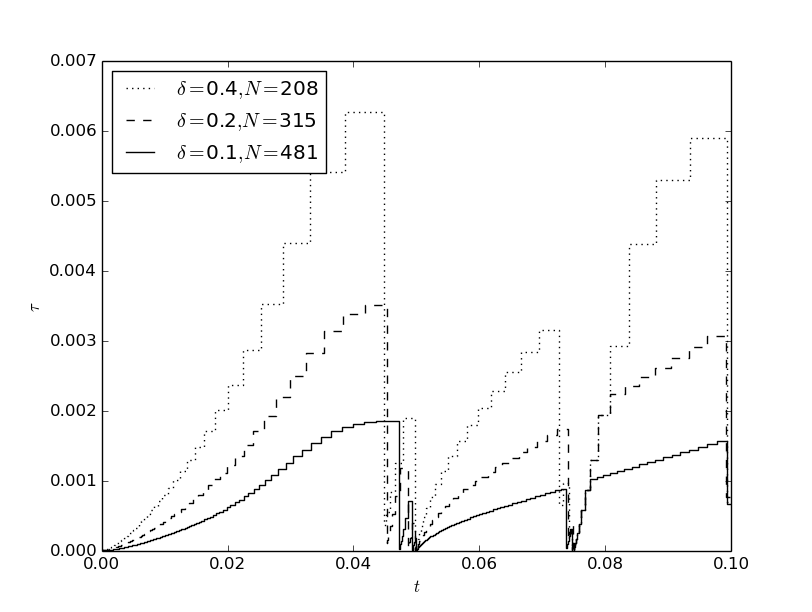
\includegraphics[width=0.5\linewidth] {art/2-1.png}
    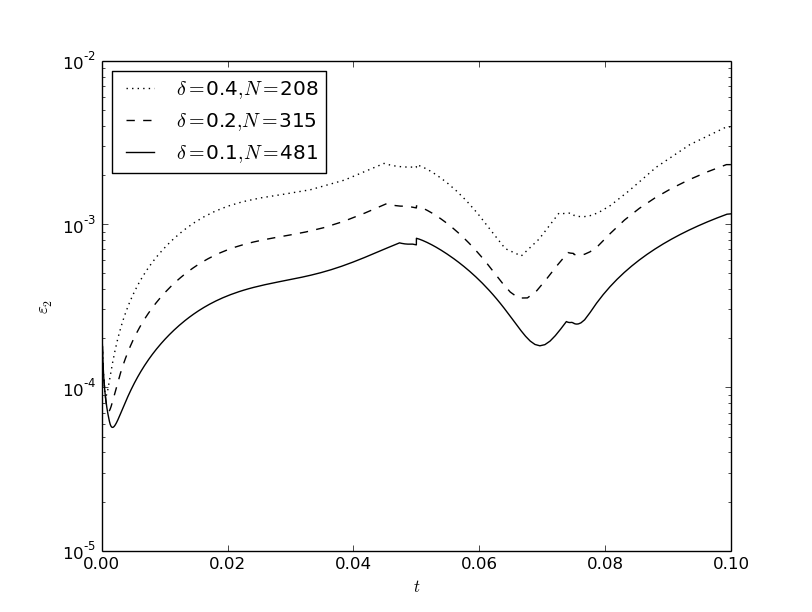
\includegraphics[width=0.5\linewidth] {art/2-2.png}
	\caption{Time steps and error in $L_2(\omega)$ on a irregular grid}
	\label{fig:2}
\end{figure}

First, we estimate the error of the approximate solution when using uniform grids on time. 
Figure \ref{fig:1} shows the dependence of the accuracy in the norm of $L_2(\omega)$ (on left) and in $L_\infty(\omega)$ (on right).
The above data demonstrate the error decreasing at the beginning of the calculation process and the error increasing at the point $t=0.05$ (the discontinuity of the right-hand side of $f(t)$) and at the point $t=0.075$ (the discontinuity of the lowest coefficient of the equation $p(t)$ ).
A successful strategy for selecting a time step should capture the noted features: a calculation with a small time step in the vicinity of $t=0$ and  $t=0.05$, $t=0.075$.

\begin{figure}[h]
    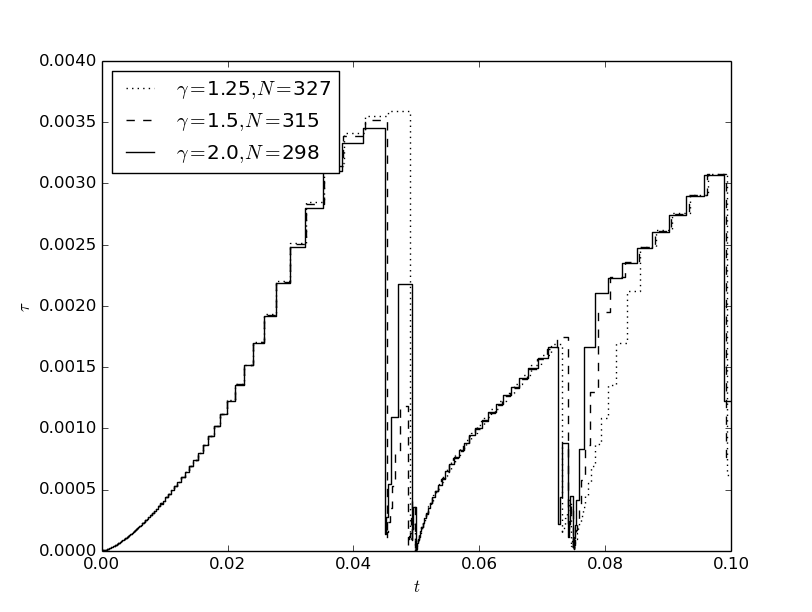
\includegraphics[width=0.5\linewidth] {art/3-1.png}
    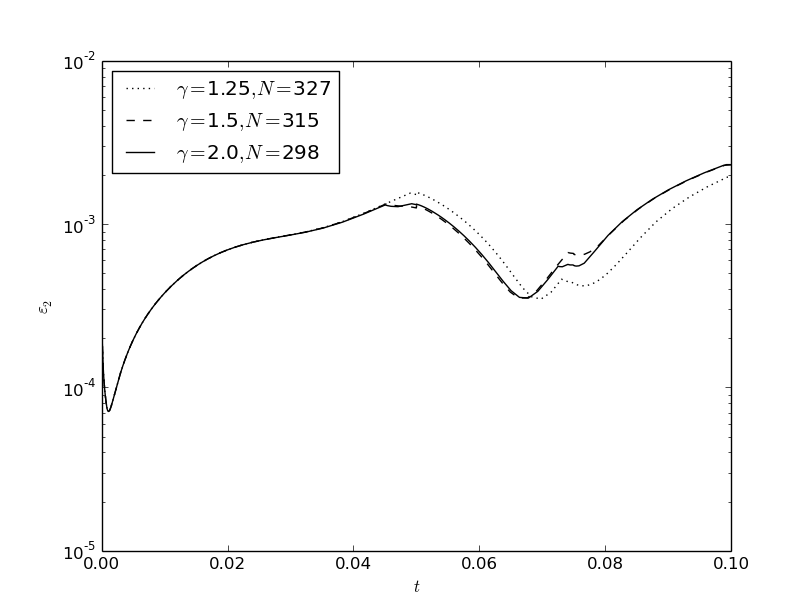
\includegraphics[width=0.5\linewidth] {art/3-2.png}
	\caption{Time steps and error for different $\gamma$}
	\label{fig:3}
\end{figure} 

The approximation error estimate is determined taking into account that $T=0.1$ and the approximate solution is determined on a unit interval in $x$. Amplitude of the solution has order 1.
Figure \ref{fig:2} shows the time steps and the errors in the norm $L_2(\omega)$  for various values of the parameter $\delta$ .
For the time step increase parameter put $\gamma=1.5$.
The calculation begins with a small step and then it gradually increases.
in the vicinity of $t=0.05$ we see a transition to essentially smaller step and a time step is also reset in the vicinity of $t=0.075$.
The accuracy of the approximate solution increases significantly at small times. In fact there is no loss of accuracy in the vicinity of the discontinuity of the right-hand side and the coefficient of the equation.
Similar data were obtained using the $L_\infty(\omega) $ norm to estimate the approximation error.
Thus, the time stepping algorithm works by selecting different norms for estimating the approximation error.

\begin{figure}[h]
    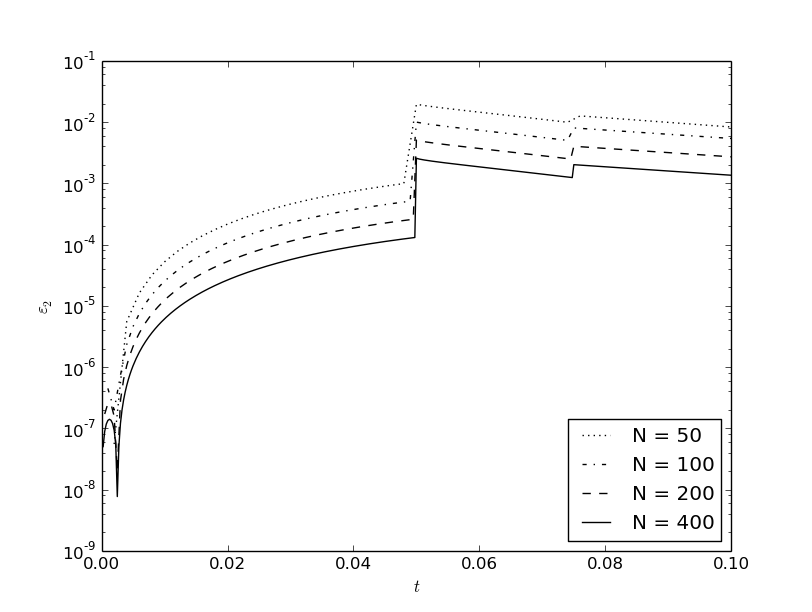
\includegraphics[width=0.5\linewidth] {art/4.png}
	\caption{The error at $\sigma = 1$ on a uniform grid}
	\label{fig:4}
\end{figure} 
\begin{figure}[h]
    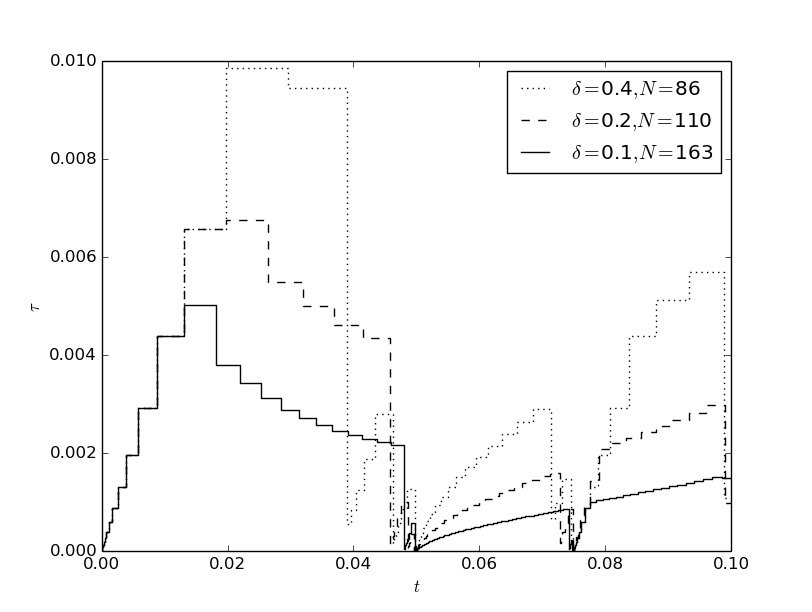
\includegraphics[width=0.5\linewidth] {art/5-1.png}
    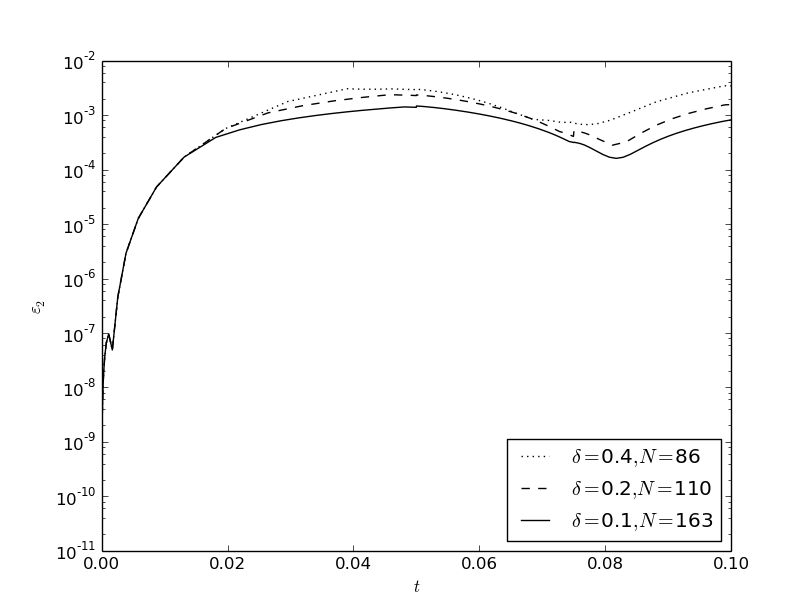
\includegraphics[width=0.5\linewidth] {art/5-2.png}
	\caption{Time steps and error at $\sigma = 1$ on a irregular grid}
	\label{fig:5}
\end{figure} 
Among the basic parameters of the proposed algorithm we can note $\gamma$ that is associated with the evaluation of the predicted step.
As shown in figure \ref{fig:3} the effect of increasing of parameter $\gamma$ is insignificant. 
Special attention should be paid on the effect of the initial conditions -- the parameter $\sigma$.
A typical situation is the presence of a boundary layer which requires the use of a fine step at small times.
For $\sigma=1$, we have a more favorable situation with an error for small $t$ (see figure \ref{fig:4}).
The irregular grid and the accuracy of the approximate solution are shown in Fig. \ref{fig:5}.
In this case the error in the initial part of the process is small.
The influence of other parameters of the problem ($\lambda$ and $\chi$) is not so significant.


% Acknowledgement
\section{ACKNOWLEDGMENTS}
This work was supported by the Russian Foundation for Basic Research (grants \#16-08-01215 and \#18-31-00315). 

% References

\nocite{*}
\bibliographystyle{aipnum-cp}%
\bibliography{vasilev}%


\end{document}
